\documentclass[a4paper,11pt]{article}

\usepackage[french]{babel}
\usepackage[T1]{fontenc}
\usepackage[utf8]{inputenc}
\usepackage{graphicx}
%\usepackage{fullpage}

\begin{document}

\title{\textbf{From Scratch to PlayStore}\\Proposition de concept}
\author{Thibaut Castanié, Noé Le Philippe, Stéphane Wouters}
\date{Master IMAGINA}
\pagestyle{empty}
\maketitle
\thispagestyle{empty}
\pagebreak 
Voici les différentes idées de concept que nous avons eues jusqu’ici. A noter qu’elles ne sont pas arrêtées et sont donc susceptibles d’être modifiées ou améliorées à tout moment jusqu'à la conception finale du cahier des charges.
\section{Idées de gameplay}
Nous voulons que notre jeu comprenne les éléments de gameplay suivants :
\begin{itemize}
\item{Gameplay de style runner}
\item{Système de jeu de type "Die \& Retry" addictif}
\item{Génération procédurale de contenu. Il nous semble plus intéressant de nous concentrer sur l’écriture d’un algorithme de génération aléatoire plutôt que consacrer du temps à la conception de niveaux.}
\item{L'expérience de jeu est basée sur la musique, c’est elle qui sera générée de façon procédurale à l’aide d’un système de \textsl{sample}. Les niveaux seront générés en fonction de la musique.
}
\end{itemize}
Pour le moment, nous voulons que le joueur manipule la mascotte du jeu (probablement un escargot avec une lunette de soleil sur chaque œil) sur la surface d’une planète. Le joueur avance en rythme avec la musique et doit franchir les obstacles qui apparaissent devant lui. Si il rate un obstacle, une valeur est décrémentée en fonction de son échec. Au fur et à mesure de la distance parcourue, le jeu devient de plus en plus dur en accélérant la vitesse de défilement de la planète, et en augmentant la difficulté des obstacles à franchir. Pendant la partie, le joueur peut récupérer des pièces qui serviront de monnaie (voir partie 3) dans la boutique.
\linebreak 
\begin{center}
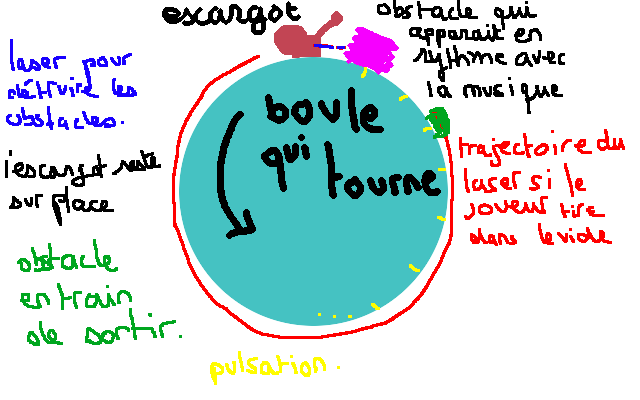
\includegraphics[width=10cm]{ter.png} 
\end{center}

\section{Style graphique}
Nous avons la volonté d’utiliser un style graphique propre et minimaliste. Les objets seront composés de formes géométriques simples, avec des couleurs vives. Nous pouvons ainsi rapidement obtenir un environnement dans un style cartoon qui rend très bien sur mobile et tablettes.
\linebreak 
\begin{center}
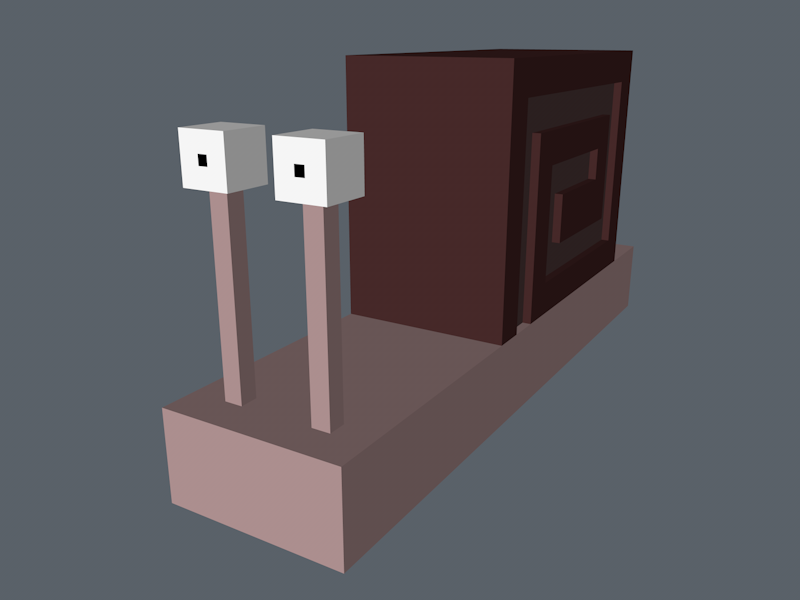
\includegraphics[width=4cm]{Escargal.png} 
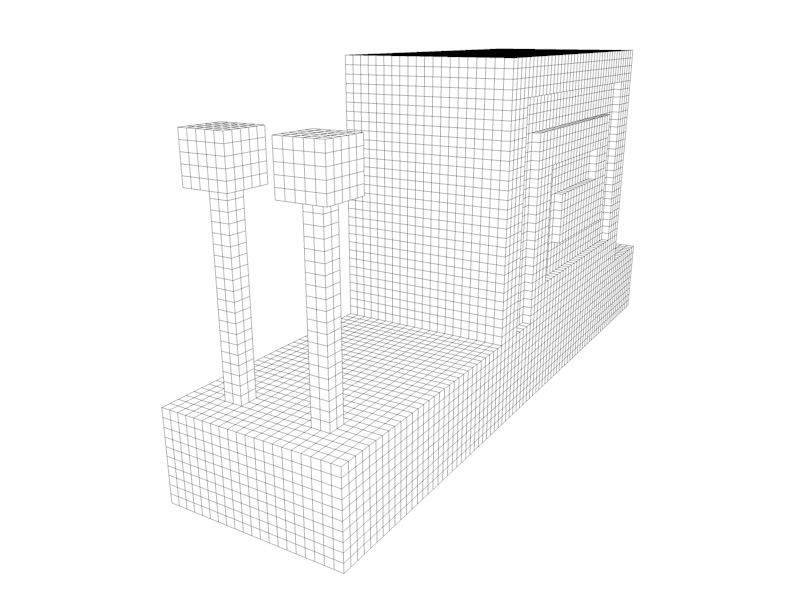
\includegraphics[width=4cm]{EscargalCellulo.png} 
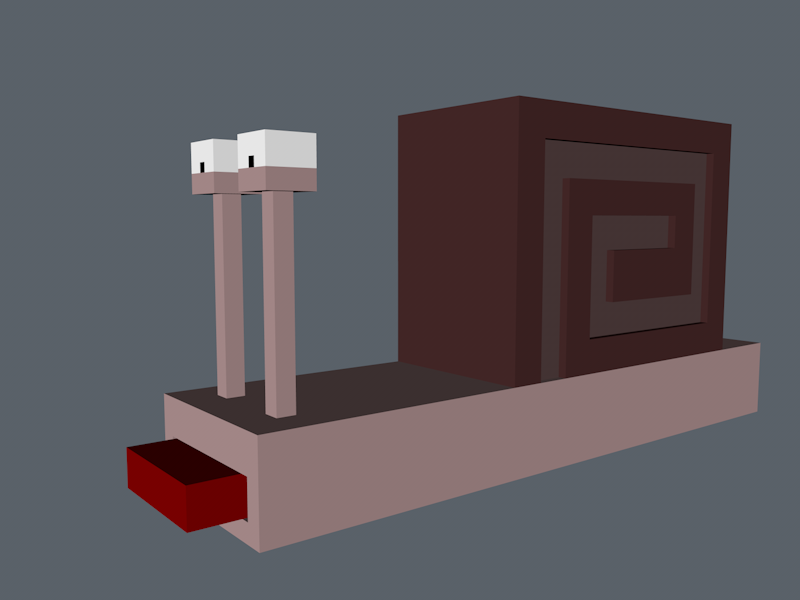
\includegraphics[width=4cm]{Escargal2.png} 
\end{center}
\begin{center}
\textsl{Prototype de mascotte}
\end{center}
\medskip
Le jeu sera en 3D mais avec le gameplay d’un jeu de plateformes 2D. Cela permet de profiter de la puissance du moteur d’Unity, en plus de rajouter un effet plus réaliste à l’univers.
\begin{center}
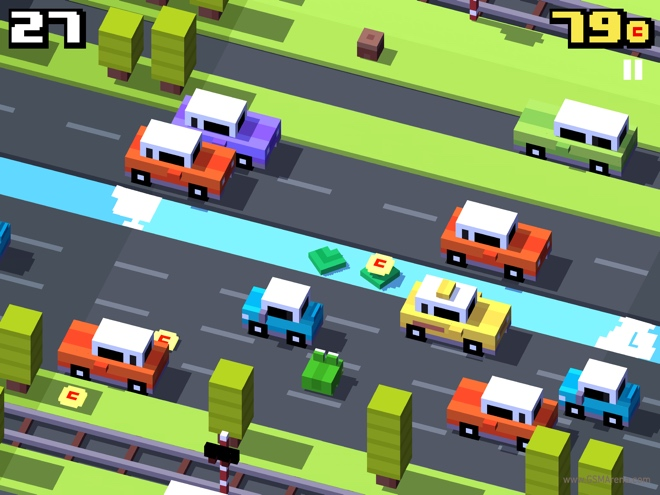
\includegraphics[width=6cm]{gsmarena_0031.jpg} 
\end{center}
\begin{center}
\textsl{Exemple de style graphique (capture de Crossy Road)}
\end{center}

\section{Monétisation}
Nous avons plusieurs façon de monétiser notre application. La première étant de placer une barrière de publicité rémunératrice, avec la possibilité pour l’utilisateur de payer pour avoir une version de l’application sans pub. La seconde façon est d’intégrer une boutique permettant d’acheter des skins pour notre personnage ou des boosts/améliorations temporaires. Ceux-ci peuvent être achetés grâce à de l’argent récupéré en jeu. Il suffit alors de rajouter une interface permettant d’acheter différents packs contenant une certaine somme d’argent “in-game”. Le développement d’une plateforme de paiement est très simplifié car il suffit d’utiliser le module de paiement “in-app” de Google.
\linebreak
La première solution a le mérite d’être rapide à mettre en place et sera rentable si notre jeu devient viral. La seconde nécessite plus de travail mais le choix de l’utilisateur sera respecté et son espace de jeu ne sera pas pollué. De plus, ce serait un moyen aux utilisateur de “récompenser” directement les développeurs, ainsi on ne leur force pas la main. Le jeu nécessite d’être addictif pour qu’une boutique “in-game” fonctionne pleinement.


\section{Unity}
Bien que nous n’ayons jamais réalisé de projet complet sous Unity, nous pensons que ce projet de TER serait un excellent moyen de maîtriser cet outil qui est très utilisé pour le développement de jeux multi-plateformes.
Depuis que nous avons émis le souhait de réaliser ce projet, nous avons commencé à développer quelques projets de test avec Unity, en nous aidant de tutoriels sur Internet, afin de gagner un peu de temps sur la phase de développement.


\section*{}
Vivre le développement d’une application mobile, de son concept jusqu’à sa publication sur le marché est une expérience très enrichissante. En effet, nous avons déjà participé à différents projets durant nos études qui nous ont permis d’améliorer nos compétences en programmation et en travail d’équipe, mais ces projets n’ont jamais inclus la mise en production du produit développé ainsi que son aspect commercial. Nous sommes donc très motivés pour réaliser ce sujet de TER.

\end{document}